\documentclass[12pt]{report}

\usepackage{xtab}

\usepackage[
  letterpaper,
  margin=0.5in,
  twocolumn,
]{geometry}

% General spacing settings

%\usepackage{setspace}
%\setstretch{}

%\setlength{\parindent}{0pt}
%\setlength{\parskip}{6pt plus 2pt minus 1pt}
%\setlength{\emergencystretch}{3em}  % prevent overfull lines

% IMPORTANT: remember to use this if lists are present
%\providecommand{\tightlist}{%
%  \setlength{\itemsep}{0pt}\setlength{\parskip}{0pt}}

% Math extensions

%\usepackage{amssymb,amsmath}

% Font selection

\usepackage{fontspec}
\setmainfont{Droid Serif}
\setsansfont{Alegreya SC}
\setmonofont{Alegreya SC}

% Hyperlinks

\usepackage[
  unicode=true
]{hyperref}

\hypersetup{
  % this will need a bit of cleanup
  breaklinks=true,
  bookmarks=true,
  pdfauthor={J. Random Author},
  pdftitle={My Magnum Opus},
  colorlinks=true,
  citecolor=blue,
  urlcolor=blue,
  linkcolor=magenta,
  pdfborder={0 0 0},
}

% don't use monospace font for urls
\urlstyle{same}

% Page headers/footers

\usepackage{fancyhdr}
\pagestyle{fancy}
\pagenumbering{arabic}
\lhead{\itshape My Magnum Opus}
\chead{}
\rhead{\itshape{\nouppercase{\leftmark}}}
\lfoot{v }
\cfoot{}
\rfoot{\thepage}

% Language selection

\usepackage{polyglossia}
\setmainlanguage{english}

% Table packages

\usepackage{longtable,multicol,booktabs}

% Graphics

%
% Ugly paragraph hack

%\ifx\paragraph\undefined\else
%\let\oldparagraph\paragraph
%\renewcommand{\paragraph}[1]{\oldparagraph{#1}\mbox{}}
%\fi
%\ifx\subparagraph\undefined\else
%\let\oldsubparagraph\subparagraph
%\renewcommand{\subparagraph}[1]{\oldsubparagraph{#1}\mbox{}}
%\fi

% Background image

\usepackage{eso-pic}
\usepackage{tikz}
\usetikzlibrary{positioning}

\AddToShipoutPicture{
%\tikz [overlay, remember picture] \node at (current page.center) {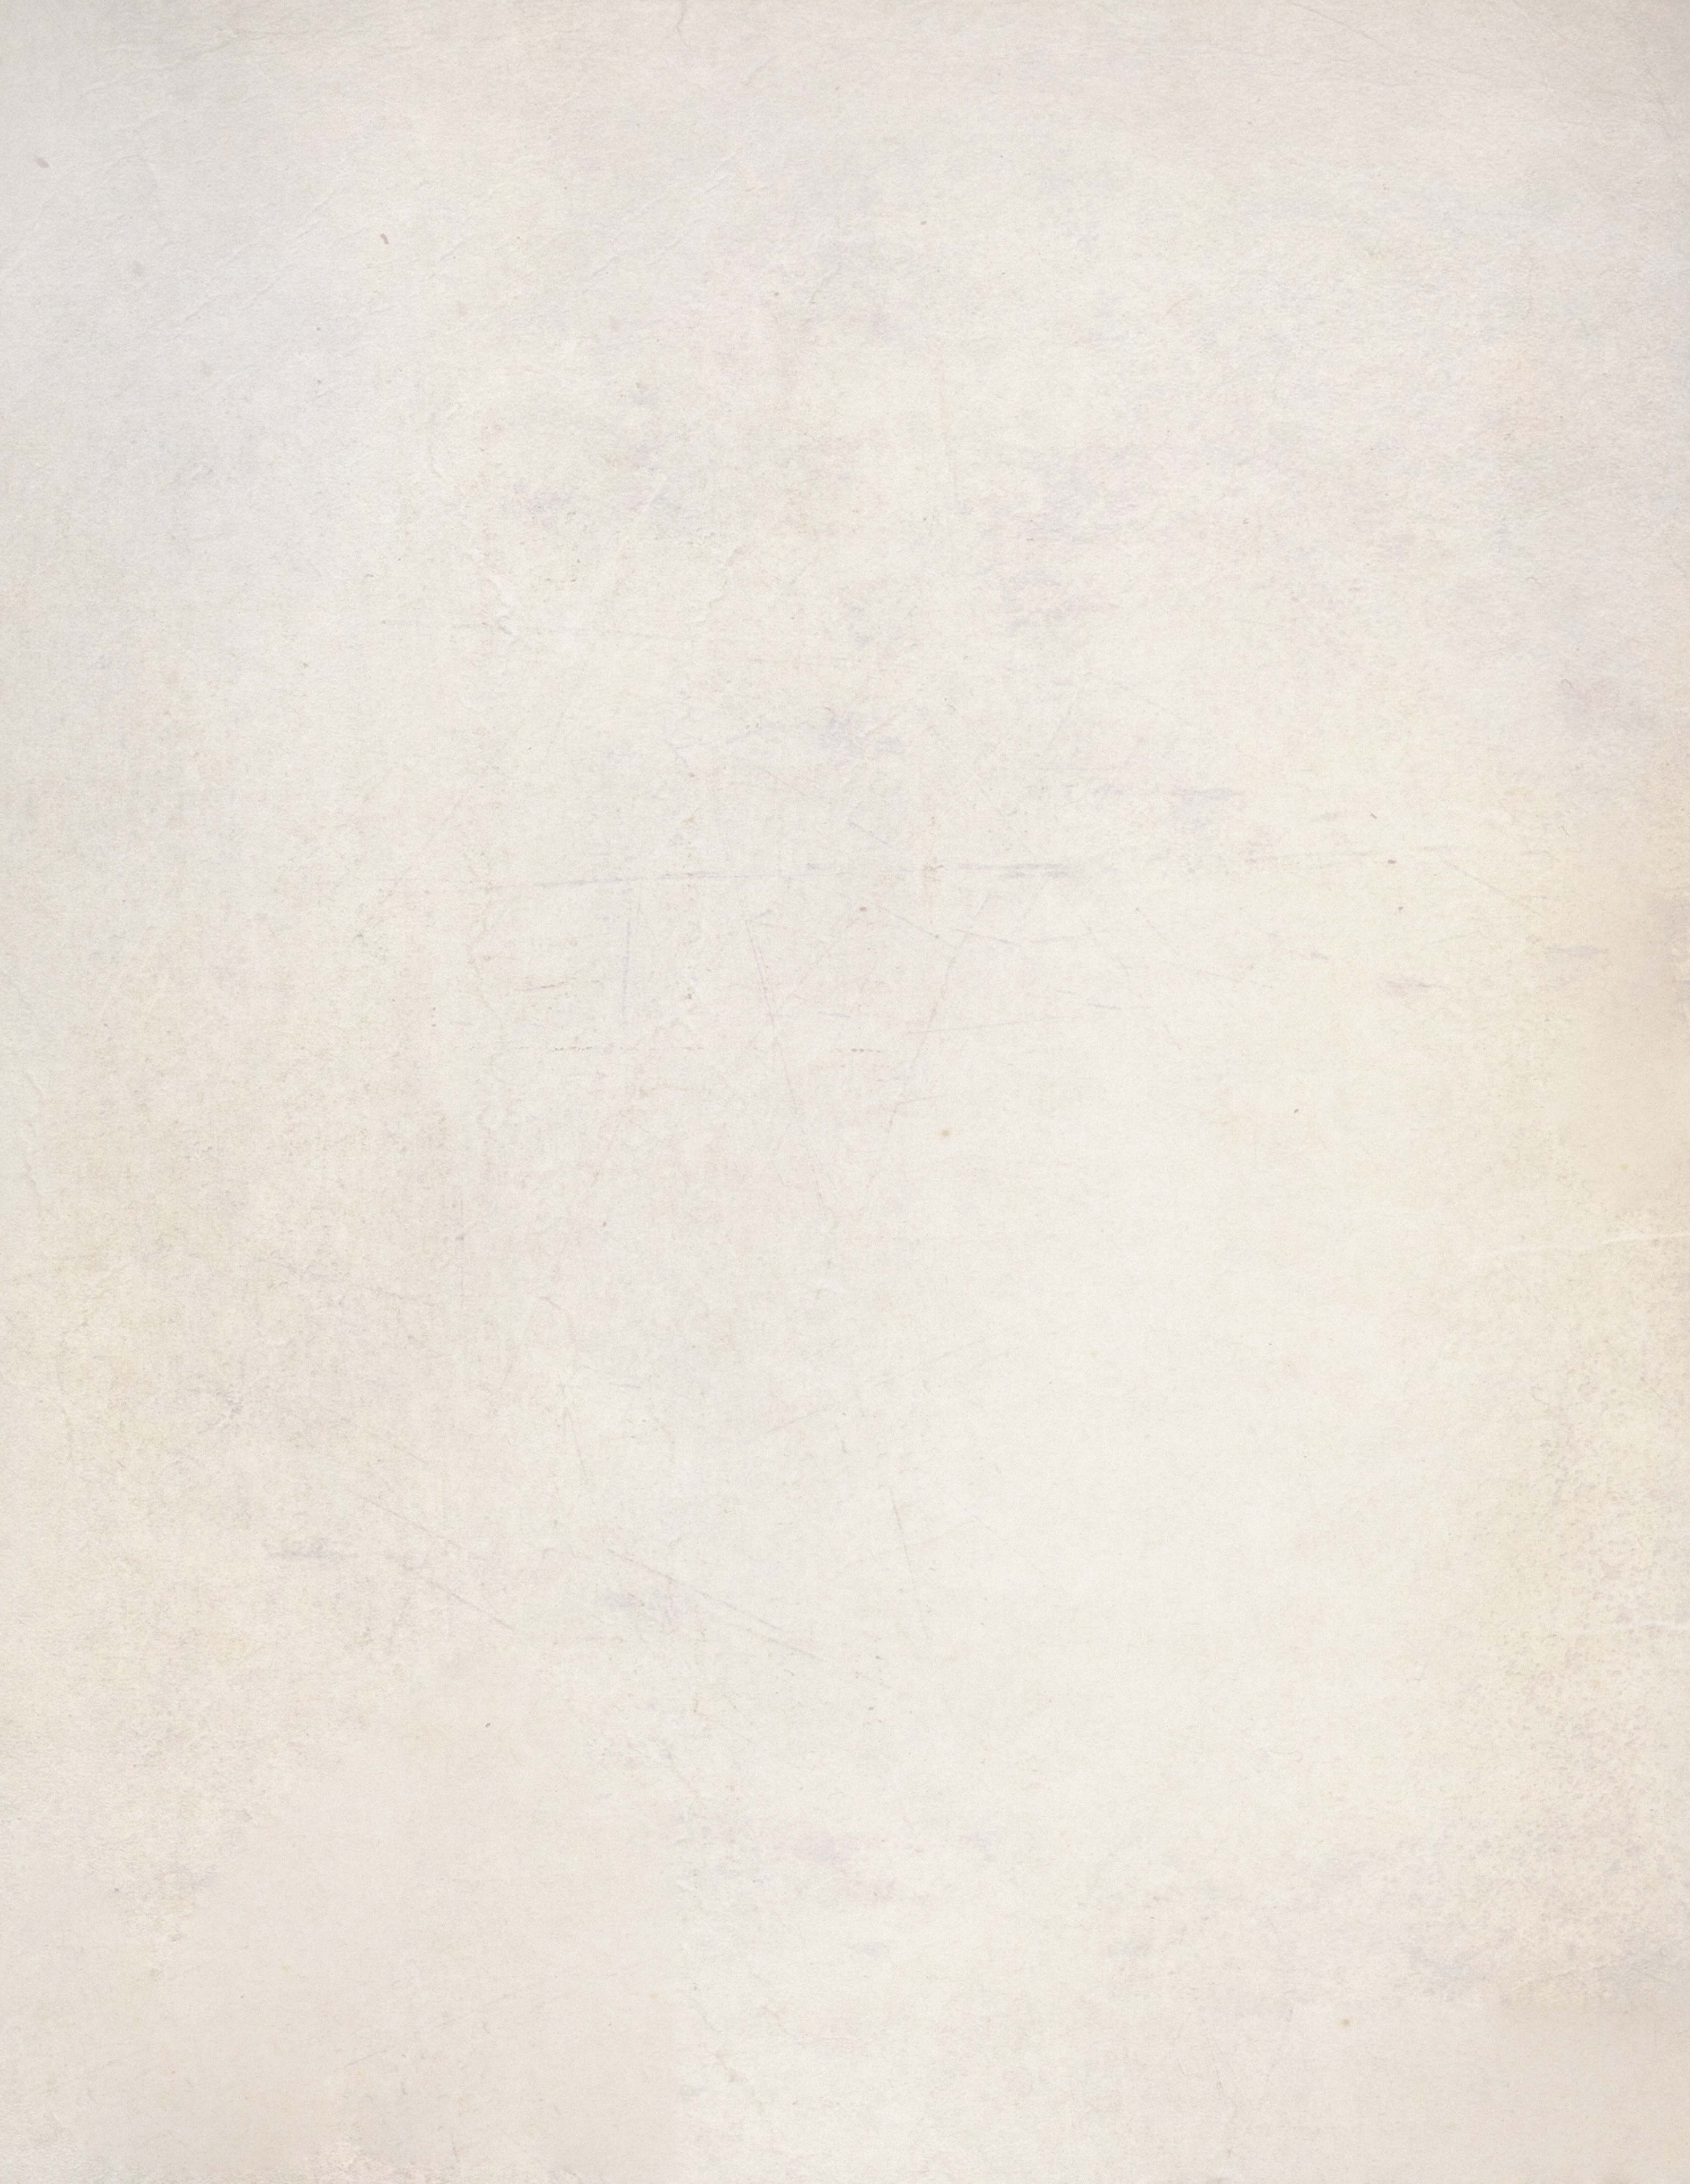
\includegraphics[width=\paperwidth,height=\paperheight,keepaspectratio]{assets/paper-bg.jpg}};
}

% Microtype

\usepackage{microtype}

% Main document

\title{My Magnum Opus}

\author{J. Random Author}

\date{}

\begin{document}
\maketitle
{
\hypersetup{linkcolor=black}
\setcounter{tocdepth}{2}
\tableofcontents
}
%\listoftables
%\listoffigures
\chapter{Chapter 1: Character
Creation}\label{chapter-1-character-creation}

Before you can start telling your story, you'll need a character to
play. This chapter will offer you step-by-step instructions to creating
your own hero. In \emph{Open Legend}, you typically begin as a level one
character. As you complete quests and gain more experience adventuring,
you'll level up and gain more power. These rules explain how to create a
character starting at level one. Later, you'll learn what to do when you
level up.

Before reading on, take a minute and think of your favorite fantasy
movies, books, or video games.

\emph{Who were the characters you identified with?}

\emph{Who inspired you?}

Now that you've got some of your favorites in mind, let's create your
character.

\subsection{Choose an Example Character \& Modify
It}\label{choose-an-example-character-modify-it}

For anyone who feels they could benefit from some inspiration, you can
easily make a copy of any of these spreadsheets (they include formulas
for doing most all of the calculations for you), and then increase or
decrease attribute scores, as well as add or remove feats. Be sure to
adjust the \textbf{Level} field to get the correct calculations for
attribute \& feat points at your current character level.

\href{https://drive.google.com/drive/u/0/folders/0Bx_UrXHMi3wmUlJjbDZiaGtIX00}{\textbf{View
Pre-generated Character Options}}

\section{Step 1: Choose Attributes}\label{step-1-choose-attributes}

Attributes are the backbone of every character in \emph{Open Legend}.
They define what your character can and can't do--the spheres he excels
in, as well as his greatest weaknesses. Whenever your character attempts
a heroic action in Open Legend, you'll look to your attributes to see
how well you succeed or fail.

In \emph{Open Legend}, attributes are divided into four categories:
physical, social, mental, and supernatural.

A character's skill with each attribute is expressed as a score from 0
(completely unpracticed) to 9 (superhuman). The average commoner or
craftsmen usually has scores ranging from 1 - 3 in several physical,
social, and mental attributes. Supernatural attributes are generally
reserved for characters of power and note.

The Attributes at a Glance tables provide a quick overview of some of
the common actions that each attribute will help you accomplish.

\begin{center}\rule{0.5\linewidth}{\linethickness}\end{center}

\textbf{Physical Attributes at a Glance}

\begin{table}

   \begin{xtabular*}{\linewidth}{@{\extracolsep{\fill}}|*{5}{p{1.2cm}|}}

      \hline

     a & b & c & d & e \\

   \end{xtabular*}

\end{table}

\begin{xtabular*}{\linewidth}{ll}
\toprule
\textbf{Agility}
&
Dodge attacks, move with stealth, perform acrobatics, shoot a bow, pick
a pocket
\tabularnewline
\textbf{Fortitude}
&
Wear heavy armor, resist poison, shrug off pain, exert yourself
physically
\tabularnewline
\textbf{Might}
&
Swing a maul, jump over a chasm, break down a door, wrestle a foe to
submission
\tabularnewline
\bottomrule
\end{xtabular*}

\end{document}
